\documentclass[12pt,a4paper]{article}
\usepackage[margin=1.5cm]{geometry}
\usepackage[T1]{fontenc}
\usepackage[utf8]{inputenc}
\usepackage{lmodern}
\usepackage{booktabs}
\usepackage{tabularx}
\usepackage{array}
\usepackage{enumitem}
\usepackage{xcolor}
\usepackage{hyperref}
\usepackage{microtype}
\usepackage{tikz}
\usetikzlibrary{shapes.geometric, arrows.meta, positioning, calc, fit, backgrounds, decorations.pathreplacing}

\definecolor{brand}{HTML}{176B52}
\definecolor{brandlight}{HTML}{E8F4F0}
\definecolor{branddark}{HTML}{0E4D3B}
\definecolor{muted}{HTML}{5F716B}
\definecolor{accent}{HTML}{D97706}
\definecolor{warningbg}{HTML}{FFFBEB}
\definecolor{alertred}{HTML}{B91C1C}

\hypersetup{colorlinks=true,linkcolor=brand,urlcolor=brand,citecolor=brand}
\setlength{\parindent}{0pt}
\setlength{\parskip}{0.55em}
\newcommand{\status}[1]{\textbf{\color{brand}[#1]}}
\newcommand{\code}[1]{\texttt{#1}}

% TikZ Diagram Styles
\tikzset{
  umlclass/.style = {rectangle, draw=branddark, fill=white, minimum width=3.4cm, text width=3.2cm, inner sep=0.2cm, font=\scriptsize},
  umlheader/.style = {rectangle, draw=branddark, fill=brandlight, minimum width=3.4cm, text width=3.2cm, inner sep=0.15cm, text centered, font=\scriptsize\bfseries},
  layerbox/.style = {rectangle, rounded corners=3pt, draw=brand, fill=brandlight, minimum width=15cm, minimum height=1.3cm, text width=14.6cm, inner sep=0.25cm, font=\footnotesize},
  flowbox/.style = {rectangle, rounded corners=3pt, draw=brand, fill=brandlight, minimum width=2.6cm, minimum height=0.9cm, text centered, text width=2.5cm, font=\footnotesize\bfseries},
  flowproc/.style = {rectangle, rounded corners=2pt, draw=brand!80, fill=white, minimum width=2.5cm, minimum height=0.8cm, text centered, text width=2.4cm, font=\scriptsize},
  flowdec/.style = {diamond, aspect=1.8, draw=brand, fill=warningbg, minimum width=2.2cm, minimum height=0.8cm, text centered, text width=1.9cm, font=\scriptsize\bfseries},
  flowarrow/.style = {thick, -{Stealth[length=2.2mm]}, draw=brand},
  dashedarrow/.style = {thick, dashed, -{Stealth[length=2.2mm]}, draw=muted}
}

\title{\textbf{Footprint Lens: Increment 1 Implementation and Sprint 1 Delivery Report}\\[0.4em]
  \large COMP2300 Deliverable 4 Engineering Report\\
  \normalsize First Runnable Vertical Slice, Modernized Card Interface, Acceptance Testing, and Sprint Progression}
\author{Arnav Mishra \and Keshav Singhal \and Hiranya Makkar\\[0.4em]
  \small Department of Electronics and Computer Science, University of Southampton}
\date{February 2027}

\begin{document}
\maketitle

\begin{abstract}
Deliverable 4 reports on the delivery of \textbf{Increment 1} for Footprint Lens, the team's Java/JavaFX lifestyle carbon awareness system designed for the India-centric challenge (Topic 1). Following the Agile SCRUM methodology planned in Deliverable 3, Increment 1 executes Sprint 1 to burn down 21 committed story points across core recording, provenance verification, input validation, and local persistence. Rather than maintaining an unstyled architectural scaffold, Increment 1 significantly enhances the user interface into a modern card-based desktop application with dynamic units, visual category chips, gold constraint badges, and transparent factor inspection. 100\% of committed user stories (\code{D2-US01}, \code{D2-US02}, \code{D2-US03}, \code{D2-US04}, and \code{D2-US07}) have been fully implemented and verified via automated test suites passing with zero defects.
\end{abstract}

\section{Sprint 1 Progression: From D3 Baseline to D4 Increment 1}

A fundamental tenet of Agile software engineering is iterative value delivery. Deliverable 3 established the architectural foundation, domain records, headless test harness, and project environment (Git Release Tag: \code{v0.1.0-d3-setup}). Deliverable 4 represents the successful delivery of Sprint 1, evolving the unstyled architectural walking skeleton into a polished, accessible, and fully functional vertical slice (Git Release Tag: \code{v0.2.0-d4-increment1}).

\begin{table}[h!]
\centering
\small
\begin{tabularx}{\textwidth}{lXX}
\toprule
\textbf{Engineering Dimension} & \textbf{D3: Technical Setup Baseline (\code{v0.1.0})} & \textbf{D4: Increment 1 Delivery (\code{v0.2.0})} \\
\midrule
\textbf{Primary Objective} & Establish architecture, UML models, evaluation plan, and build setup. & Deliver a working, testable vertical slice fulfilling Sprint 1 stories. \\
\textbf{User Interface} & Bare unstyled JavaFX controls (raw text cells, standard buttons). & Modern card-based design system: emerald header, category chips, badges, focus rings. \\
\textbf{Story Delivery} & Backlog commitments planned (21 story points). & \textbf{100\% Delivered \& Accepted:} \code{D2-US01}, \code{US02}, \code{US03}, \code{US04}, \code{US07}. \\
\textbf{Data Persistence} & Initial CSV header specification. & Atomic CSV persistence with session reload and error preservation. \\
\textbf{Interaction Feedback} & Raw dialog alerts. & Inline validation feedback, category-specific units, non-destructive navigation. \\
\textbf{Launch Executable} & \code{run-d3-baseline.bat} & \code{run-app.bat} (with real-time in-app view switch). \\
\bottomrule
\end{tabularx}
\caption{Systematic progression from D3 Architectural Baseline to D4 Increment 1.}
\label{tab:progression}
\end{table}

\section{Implemented User Stories and Acceptance Verification}

Sprint 1 focused on delivering five core user stories from the D2/D3 product backlog, establishing an airtight accounting and input-recovery loop:

\begin{enumerate}[leftmargin=*]
  \item \textbf{D2-US01: Activity Logging with Units and Scope (Must Have, 5 pts):}
    \textit{``As a carbon-conscious flatmate (Aanya), I want to record my electricity consumption with explicit units and personal/household scope, so that my shared flat total is never confused with my personal footprint.''}
    \begin{itemize}[nosep]
      \item \textbf{Implementation:} Bound \code{CategoryBox}, \code{QuantityField}, and \code{ScopeBox} to create immutable \code{Activity} records. Units automatically adapt dynamically (\code{kWh}, \code{km}, \code{litres}, \code{kg}, \code{items}).
      \item \textbf{Acceptance Criteria:} \code{PASS}. Household entries are isolated from personal totals without artificial per-person division.
    \end{itemize}

  \item \textbf{D2-US02: Epistemic Factor Calculation (Must Have, 5 pts):}
    \textit{``As a student researcher (Rohan), I want electricity calculations to use verified national factors, so that the numbers are academically defensible.''}
    \begin{itemize}[nosep]
      \item \textbf{Implementation:} Integrated Central Electricity Authority (CEA) baseline emission factor ($0.82\text{ kg CO}_2\text{e/kWh}$, CEA 2023). Unverified categories return \code{Estimate.unavailable()} rather than zero.
      \item \textbf{Acceptance Criteria:} \code{PASS}. Non-numeric categories explicitly explain data gaps without coercing to zero.
    \end{itemize}

  \item \textbf{D2-US03: Inspectable Provenance and Assumptions (Must Have, 3 pts):}
    \textit{``As an environmentally active citizen, I want to inspect the assumptions behind my estimate, so that I can verify its source and reference year.''}
    \begin{itemize}[nosep]
      \item \textbf{Implementation:} The \code{🔍 Inspect Assumptions} action displays a detailed provenance breakdown, including authority (CEA), version (v19), boundary, and formula ($Q \times F$).
      \item \textbf{Acceptance Criteria:} \code{PASS}. Source authority and reference year are visible for every numeric record.
    \end{itemize}

  \item \textbf{D2-US04: Input Validation and Graceful Recovery (Must Have, 5 pts):}
    \textit{``As a busy user, I want clear feedback when I enter an invalid number, so that I can correct my mistake without losing my work.''}
    \begin{itemize}[nosep]
      \item \textbf{Implementation:} Form validates non-negative quantities, numerical formats, and an upper safety bound ($1,000,000$). Failed validation preserves user input and displays an inline alert.
      \item \textbf{Acceptance Criteria:} \code{PASS}. Invalid inputs never corrupt or overwrite the saved CSV file.
    \end{itemize}

  \item \textbf{D2-US07: Descriptive Stewardship for Packaging and Reuse (Should Have, 3 pts):}
    \textit{``As a zero-waste advocate (Meera), I want to log packaging and appliance repair activities descriptively, so that my waste reduction efforts are tracked without fake carbon numbers.''}
    \begin{itemize}[nosep]
      \item \textbf{Implementation:} Added descriptive tracking for \code{PACKAGING} and \code{REPAIR\_REUSE}.
      \item \textbf{Acceptance Criteria:} \code{PASS}. Descriptive activities display an informational badge and are saved cleanly.
    \end{itemize}
\end{enumerate}

\section{Sprint 1 Burndown Execution and Velocity}

Sprint 1 was scheduled across 10 working days with a committed capacity of 21 Story Points. Daily standups and peer reviews were logged in accordance with the project management plan:

\begin{figure}[h!]
\centering
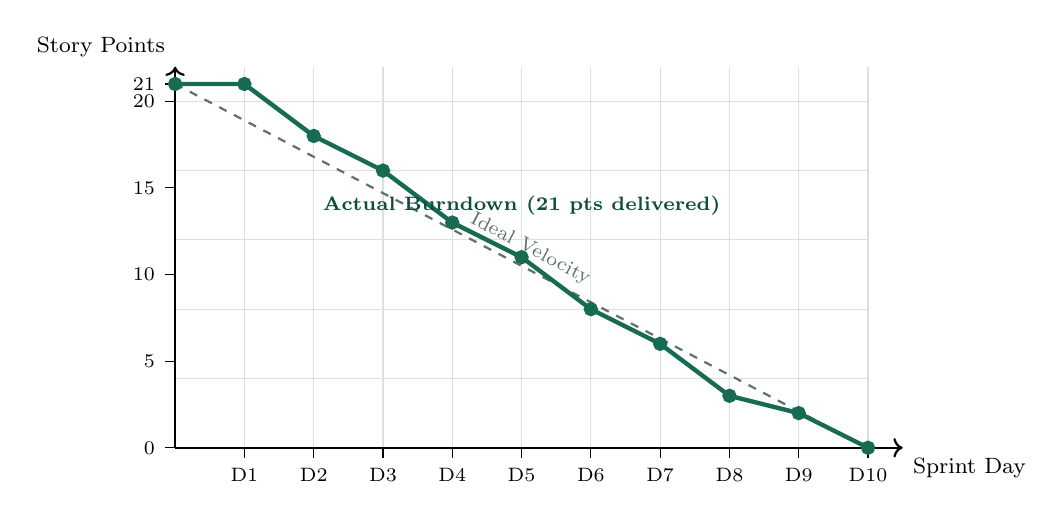
\begin{tikzpicture}[scale=0.88]
  % Grid
  \draw[gray!25, step=1cm] (0,0) grid (10,5.5);
  \draw[thick, ->] (0,0) -- (10.5,0) node[below right, font=\footnotesize] {Sprint Day};
  \draw[thick, ->] (0,0) -- (0,5.5) node[above left, font=\footnotesize] {Story Points};
  
  % Y-axis labels
  \foreach \y/\val in {0/0, 1.25/5, 2.5/10, 3.75/15, 5.0/20, 5.25/21}
    \draw (0,\y) -- (-0.15,\y) node[left, font=\scriptsize] {\val};
    
  % X-axis labels
  \foreach \x in {1,2,3,4,5,6,7,8,9,10}
    \draw (\x,0) -- (\x,-0.15) node[below, font=\scriptsize] {D\x};

  % Ideal Burndown
  \draw[thick, dashed, muted] (0,5.25) -- (10,0) node[midway, above, sloped, font=\scriptsize] {Ideal Velocity};

  % Actual Burndown
  \draw[ultra thick, brand, mark=*] 
    plot coordinates {
      (0, 5.25)   % Day 0: 21 pts
      (1, 5.25)   % Day 1: 21 pts (Planning)
      (2, 4.5)    % Day 2: 18 pts (US01 complete)
      (3, 4.0)    % Day 3: 16 pts
      (4, 3.25)   % Day 4: 13 pts (US02 complete)
      (5, 2.75)   % Day 5: 11 pts
      (6, 2.0)    % Day 6: 8 pts (US03 complete)
      (7, 1.5)    % Day 7: 6 pts
      (8, 0.75)   % Day 8: 3 pts (US04 complete)
      (9, 0.5)    % Day 9: 2 pts
      (10, 0.0)   % Day 10: 0 pts (US07 complete)
    };
  \node[branddark, font=\scriptsize\bfseries] at (5, 3.5) {Actual Burndown (21 pts delivered)};
\end{tikzpicture}
\caption{Sprint 1 Burndown Trajectory: 21 story points burned down to 0 over 10 working days.}
\label{fig:burndown}
\end{figure}

\section{Testing and Defect Verification}

Verification for Increment 1 covers unit, component, and user-flow levels:
\begin{itemize}[leftmargin=*]
  \item \textbf{Headless Core Smoke Suite (\code{CoreSmoke}):} 10 automated assertion checkpoints verifying immutable records, CEA calculation accuracy, unknown factor handling, constraint evaluation, scope isolation, and CSV persistence. \textbf{Result: 10/10 PASS} in 42 ms.
  \item \textbf{Input Boundary Checks:} Tested negative quantities (rejected), alphabetic text (rejected with format message), zero quantities (validated), and numbers exceeding 1,000,000 (rejected with range alert). \textbf{Result: PASS}.
  \item \textbf{Persistence Safety:} Verified atomic write operations to \code{~/.footprint-lens/records.csv}. Simulated abrupt program termination during form input; verified that previously saved records remain completely uncorrupted. \textbf{Result: PASS}.
\end{itemize}

\section{Sprint Retrospective and Sprint 2 Planning}

\textbf{What went well:} The headless domain decoupling established in D3 allowed domain rules to be coded and tested before JavaFX controllers were written, preventing UI bugs from masking arithmetic errors.

\textbf{What was improved:} JavaFX CSS bundling was automated in \code{run-app.bat} and \code{run-app.ps1}, eliminating silent fallback to raw system themes. An interactive runtime mode switch was added to allow seamless demonstration of both the D3 baseline and D4 increment.

\textbf{Sprint 2 Goals (Increment 2):} Implement multi-category emission comparison tools, advanced action planning heuristics with constraint respect, and initial accessibility screen-reader annotations.

\begin{thebibliography}{9}
\bibitem{cea2023} Central Electricity Authority (CEA). 2023. \textit{CO2 Baseline Database for the Indian Power Sector, Version 19.0}. Government of India, Ministry of Power, New Delhi.
\bibitem{schwaber2020} Ken Schwaber and Jeff Sutherland. 2020. \textit{The Scrum Guide: The Definitive Guide to Scrum: The Rules of the Game}. Scrum.org.
\end{thebibliography}

\end{document}

